\documentclass[twoside]{book}

% Packages required by doxygen
\usepackage{fixltx2e}
\usepackage{calc}
\usepackage{doxygen}
\usepackage[export]{adjustbox} % also loads graphicx
\usepackage{graphicx}
\usepackage[utf8]{inputenc}
\usepackage{makeidx}
\usepackage{multicol}
\usepackage{multirow}
\PassOptionsToPackage{warn}{textcomp}
\usepackage{textcomp}
\usepackage[nointegrals]{wasysym}
\usepackage[table]{xcolor}

% Font selection
\usepackage[T1]{fontenc}
\usepackage[scaled=.90]{helvet}
\usepackage{courier}
\usepackage{amssymb}
\usepackage{sectsty}
\renewcommand{\familydefault}{\sfdefault}
\allsectionsfont{%
  \fontseries{bc}\selectfont%
  \color{darkgray}%
}
\renewcommand{\DoxyLabelFont}{%
  \fontseries{bc}\selectfont%
  \color{darkgray}%
}
\newcommand{\+}{\discretionary{\mbox{\scriptsize$\hookleftarrow$}}{}{}}

% Page & text layout
\usepackage{geometry}
\geometry{%
  a4paper,%
  top=2.5cm,%
  bottom=2.5cm,%
  left=2.5cm,%
  right=2.5cm%
}
\tolerance=750
\hfuzz=15pt
\hbadness=750
\setlength{\emergencystretch}{15pt}
\setlength{\parindent}{0cm}
\setlength{\parskip}{3ex plus 2ex minus 2ex}
\makeatletter
\renewcommand{\paragraph}{%
  \@startsection{paragraph}{4}{0ex}{-1.0ex}{1.0ex}{%
    \normalfont\normalsize\bfseries\SS@parafont%
  }%
}
\renewcommand{\subparagraph}{%
  \@startsection{subparagraph}{5}{0ex}{-1.0ex}{1.0ex}{%
    \normalfont\normalsize\bfseries\SS@subparafont%
  }%
}
\makeatother

% Headers & footers
\usepackage{fancyhdr}
\pagestyle{fancyplain}
\fancyhead[LE]{\fancyplain{}{\bfseries\thepage}}
\fancyhead[CE]{\fancyplain{}{}}
\fancyhead[RE]{\fancyplain{}{\bfseries\leftmark}}
\fancyhead[LO]{\fancyplain{}{\bfseries\rightmark}}
\fancyhead[CO]{\fancyplain{}{}}
\fancyhead[RO]{\fancyplain{}{\bfseries\thepage}}
\fancyfoot[LE]{\fancyplain{}{}}
\fancyfoot[CE]{\fancyplain{}{}}
\fancyfoot[RE]{\fancyplain{}{\bfseries\scriptsize Generated by Doxygen }}
\fancyfoot[LO]{\fancyplain{}{\bfseries\scriptsize Generated by Doxygen }}
\fancyfoot[CO]{\fancyplain{}{}}
\fancyfoot[RO]{\fancyplain{}{}}
\renewcommand{\footrulewidth}{0.4pt}
\renewcommand{\chaptermark}[1]{%
  \markboth{#1}{}%
}
\renewcommand{\sectionmark}[1]{%
  \markright{\thesection\ #1}%
}

% Indices & bibliography
\usepackage{natbib}
\usepackage[titles]{tocloft}
\setcounter{tocdepth}{3}
\setcounter{secnumdepth}{5}
\makeindex

% Hyperlinks (required, but should be loaded last)
\usepackage{ifpdf}
\ifpdf
  \usepackage[pdftex,pagebackref=true]{hyperref}
\else
  \usepackage[ps2pdf,pagebackref=true]{hyperref}
\fi
\hypersetup{%
  colorlinks=true,%
  linkcolor=blue,%
  citecolor=blue,%
  unicode%
}

% Custom commands
\newcommand{\clearemptydoublepage}{%
  \newpage{\pagestyle{empty}\cleardoublepage}%
}

\usepackage{caption}
\captionsetup{labelsep=space,justification=centering,font={bf},singlelinecheck=off,skip=4pt,position=top}

%===== C O N T E N T S =====

\begin{document}

% Titlepage & ToC
\hypersetup{pageanchor=false,
             bookmarksnumbered=true,
             pdfencoding=unicode
            }
\pagenumbering{alph}
\begin{titlepage}
\vspace*{7cm}
\begin{center}%
{\Large ActiveX }\\
\vspace*{1cm}
{\large Generated by Doxygen 1.8.13}\\
\end{center}
\end{titlepage}
\clearemptydoublepage
\pagenumbering{roman}
\tableofcontents
\clearemptydoublepage
\pagenumbering{arabic}
\hypersetup{pageanchor=true}

%--- Begin generated contents ---
\chapter{Hierarchical Index}
\section{Class Hierarchy}
This inheritance list is sorted roughly, but not completely, alphabetically\+:\begin{DoxyCompactList}
\item \contentsline{section}{Active\+Excel}{\pageref{class_active_excel}}{}
\item \contentsline{section}{Active\+Word}{\pageref{class_active_word}}{}
\item Q\+Main\+Window\begin{DoxyCompactList}
\item \contentsline{section}{Main\+Window}{\pageref{class_main_window}}{}
\end{DoxyCompactList}
\item \contentsline{section}{Ui\+\_\+\+Main\+Window}{\pageref{class_ui___main_window}}{}
\begin{DoxyCompactList}
\item \contentsline{section}{Ui\+:\+:Main\+Window}{\pageref{class_ui_1_1_main_window}}{}
\end{DoxyCompactList}
\end{DoxyCompactList}

\chapter{Class Index}
\section{Class List}
Here are the classes, structs, unions and interfaces with brief descriptions\+:\begin{DoxyCompactList}
\item\contentsline{section}{\hyperlink{class_active_excel}{Active\+Excel} \\*Класс для работы с excel\textquotesingle{}овскими документами при помощи Active\+Qt. Ежели функция возвращает указатель на N\+U\+LL, значит не корректная работа }{\pageref{class_active_excel}}{}
\item\contentsline{section}{\hyperlink{class_active_word}{Active\+Word} \\*Класс для работы с word\textquotesingle{}овскими документами при помощи Active\+Qt. Ежели функция возвращает указатель на N\+U\+LL, значит не корректная работа }{\pageref{class_active_word}}{}
\item\contentsline{section}{\hyperlink{class_ui_1_1_main_window}{Ui\+::\+Main\+Window} }{\pageref{class_ui_1_1_main_window}}{}
\item\contentsline{section}{\hyperlink{class_main_window}{Main\+Window} }{\pageref{class_main_window}}{}
\item\contentsline{section}{\hyperlink{class_ui___main_window}{Ui\+\_\+\+Main\+Window} }{\pageref{class_ui___main_window}}{}
\end{DoxyCompactList}

\chapter{Class Documentation}
\hypertarget{class_active_excel}{}\section{Active\+Excel Class Reference}
\label{class_active_excel}\index{Active\+Excel@{Active\+Excel}}


Класс для работы с excel\textquotesingle{}овскими документами при помощи Active\+Qt. Ежели функция возвращает указатель на N\+U\+LL, значит не корректная работа.  




{\ttfamily \#include $<$activeexcel.\+h$>$}

\subsection*{Public Member Functions}
\begin{DoxyCompactItemize}
\item 
Q\+Ax\+Object $\ast$ \hyperlink{class_active_excel_a64a459d7894744a4e879670db82692f7}{document\+Open} (Q\+Variant path=\char`\"{}\char`\"{})
\begin{DoxyCompactList}\small\item\em Открыть документ \end{DoxyCompactList}\item 
Q\+Ax\+Object $\ast$ \hyperlink{class_active_excel_ab59ba747de1ca7170d2901ac186f0b4d}{document\+Add\+Sheet} (Q\+Variant sheet\+Name=\char`\"{}\char`\"{})
\begin{DoxyCompactList}\small\item\em Возвращает указатель на созданный лист По умолчанию создается Лист1, Лист2 ... \end{DoxyCompactList}\item 
Q\+Ax\+Object $\ast$ \hyperlink{class_active_excel_a259dc8f89d7d93726c2fd9ef86a53044}{document\+Sheet\+Active} (Q\+Variant sheet)
\item 
void \hyperlink{class_active_excel_a7be6d6cfc05409fd23d9ae0dff95353b}{document\+Close} (Q\+Ax\+Object $\ast$document)
\begin{DoxyCompactList}\small\item\em Закрытие документа без сохранения. Указатель на документ будет удален внутри функции \end{DoxyCompactList}\item 
void \hyperlink{class_active_excel_ab3bf3535715a62ca818013cd9d8cd05a}{document\+Close\+And\+Save} (Q\+Ax\+Object $\ast$document, Q\+Variant path)
\begin{DoxyCompactList}\small\item\em указатель на документ будет удален внутри функции \end{DoxyCompactList}\item 
void \hyperlink{class_active_excel_ae6e242799d2be9d766f053ed01286b48}{sheet\+Cell\+Paste} (Q\+Ax\+Object $\ast$sheet, Q\+Variant string, Q\+Variant row, Q\+Variant col)
\begin{DoxyCompactList}\small\item\em Установка значения в ячейку \end{DoxyCompactList}\item 
Q\+Variant \hyperlink{class_active_excel_ad0e7d4faad5ac5b1d476b2112e835636}{sheet\+Cell\+Insert} (Q\+Ax\+Object $\ast$sheet, Q\+Variant row, Q\+Variant col)
\begin{DoxyCompactList}\small\item\em Получение значения из ячейки \end{DoxyCompactList}\item 
void \hyperlink{class_active_excel_ab2ef703bfeed8edd98005bff2fafa0b3}{sheet\+Copy\+To\+Buf} (Q\+Ax\+Object $\ast$sheet, Q\+Variant row\+Col)
\begin{DoxyCompactList}\small\item\em копирование ячеек в буфер диспазон ячейки записывается как A1\+:B13. \end{DoxyCompactList}\item 
void \hyperlink{class_active_excel_a1d363f3394905392c98e3ba78bc6588a}{sheet\+Past\+From\+Buf} (Q\+Ax\+Object $\ast$sheet, Q\+Variant row\+Col)
\begin{DoxyCompactList}\small\item\em вставка из буфера \end{DoxyCompactList}\item 
void \hyperlink{class_active_excel_a98c0020e0eabd459872b07a0247e2482}{sheet\+Cell\+Merge} (Q\+Ax\+Object $\ast$sheet, Q\+Variant row\+Col)
\begin{DoxyCompactList}\small\item\em Объединение ячеек \end{DoxyCompactList}\item 
void \hyperlink{class_active_excel_a5c4341cd4fd4eaceab92eef20991b0ab}{sheet\+Cell\+Height\+Width} (Q\+Ax\+Object $\ast$sheet, Q\+Variant Row\+Height, Q\+Variant Column\+Width, Q\+Variant row\+Col)
\begin{DoxyCompactList}\small\item\em Ширина строк и столбцов \end{DoxyCompactList}\item 
void \hyperlink{class_active_excel_a07229b0542e5fa9bbb8d795a1c84c831}{sheet\+Cell\+Horizontal\+Alignment} (Q\+Ax\+Object $\ast$sheet, Q\+Variant row\+Col, bool left=false, bool right=false, bool center=false)
\begin{DoxyCompactList}\small\item\em Выравнивание ячеек. один из 3 параметров равен true. \end{DoxyCompactList}\item 
void \hyperlink{class_active_excel_a5c0660c91b28d1d7ce550789104c90e9}{sheet\+Cell\+Vertical\+Alignment} (Q\+Ax\+Object $\ast$sheet, Q\+Variant row\+Col, bool up=false, bool down=false, bool center=false)
\begin{DoxyCompactList}\small\item\em Выравнивание ячеек. один из 3 параметров равен true. \end{DoxyCompactList}\end{DoxyCompactItemize}


\subsection{Detailed Description}
Класс для работы с excel\textquotesingle{}овскими документами при помощи Active\+Qt. Ежели функция возвращает указатель на N\+U\+LL, значит не корректная работа. 

\begin{DoxyWarning}{Warning}
При создании/ открытии документа его надо сохранить. Новому документу автоматически присваивается индекс = 1; Позиция индекса откры-\/ тых ранее документов сдвигается на 1. Не сохраненный документ называется \char`\"{}Документ\mbox{[}n\mbox{]}\char`\"{}, где n = 1 до первого открытого документа.
\end{DoxyWarning}
Совет\+: внимательно следите за создаваемыми объектами и указателями, возвращаемыми методом query\+Sub\+Object(). Они не удаляются автоматически, нужно вызывать delete вручную. В противном случае будет эффективно расходоваться память, и после нескольких тысяч вызовов метода query\+Sub\+Object() ваша программа и эксель в сумме займут всю память, но это полбеды -\/ обращение к одной ячейке будет занимать секунду. Это всего лишь предостережение...

\begin{DoxyVersion}{Version}
1.\+0 
\end{DoxyVersion}


\subsection{Member Function Documentation}
\mbox{\Hypertarget{class_active_excel_ab59ba747de1ca7170d2901ac186f0b4d}\label{class_active_excel_ab59ba747de1ca7170d2901ac186f0b4d}} 
\index{Active\+Excel@{Active\+Excel}!document\+Add\+Sheet@{document\+Add\+Sheet}}
\index{document\+Add\+Sheet@{document\+Add\+Sheet}!Active\+Excel@{Active\+Excel}}
\subsubsection{\texorpdfstring{document\+Add\+Sheet()}{documentAddSheet()}}
{\footnotesize\ttfamily Q\+Ax\+Object $\ast$ Active\+Excel\+::document\+Add\+Sheet (\begin{DoxyParamCaption}\item[{Q\+Variant}]{sheet\+Name = {\ttfamily \char`\"{}\char`\"{}} }\end{DoxyParamCaption})}



Возвращает указатель на созданный лист По умолчанию создается Лист1, Лист2 ... 

\mbox{[}in\mbox{]} имя листа \mbox{\Hypertarget{class_active_excel_a7be6d6cfc05409fd23d9ae0dff95353b}\label{class_active_excel_a7be6d6cfc05409fd23d9ae0dff95353b}} 
\index{Active\+Excel@{Active\+Excel}!document\+Close@{document\+Close}}
\index{document\+Close@{document\+Close}!Active\+Excel@{Active\+Excel}}
\subsubsection{\texorpdfstring{document\+Close()}{documentClose()}}
{\footnotesize\ttfamily void Active\+Excel\+::document\+Close (\begin{DoxyParamCaption}\item[{Q\+Ax\+Object $\ast$}]{document }\end{DoxyParamCaption})}



Закрытие документа без сохранения. Указатель на документ будет удален внутри функции 

\mbox{[}in\mbox{]} указатель на созданный документ \mbox{\Hypertarget{class_active_excel_ab3bf3535715a62ca818013cd9d8cd05a}\label{class_active_excel_ab3bf3535715a62ca818013cd9d8cd05a}} 
\index{Active\+Excel@{Active\+Excel}!document\+Close\+And\+Save@{document\+Close\+And\+Save}}
\index{document\+Close\+And\+Save@{document\+Close\+And\+Save}!Active\+Excel@{Active\+Excel}}
\subsubsection{\texorpdfstring{document\+Close\+And\+Save()}{documentCloseAndSave()}}
{\footnotesize\ttfamily void Active\+Excel\+::document\+Close\+And\+Save (\begin{DoxyParamCaption}\item[{Q\+Ax\+Object $\ast$}]{document,  }\item[{Q\+Variant}]{path }\end{DoxyParamCaption})}



указатель на документ будет удален внутри функции 


\begin{DoxyParams}[1]{Parameters}
\mbox{\tt in}  & {\em path} & путь для сохранения \\
\hline
\end{DoxyParams}
\begin{DoxyReturn}{Returns}
указатель листа 
\end{DoxyReturn}
\mbox{\Hypertarget{class_active_excel_a64a459d7894744a4e879670db82692f7}\label{class_active_excel_a64a459d7894744a4e879670db82692f7}} 
\index{Active\+Excel@{Active\+Excel}!document\+Open@{document\+Open}}
\index{document\+Open@{document\+Open}!Active\+Excel@{Active\+Excel}}
\subsubsection{\texorpdfstring{document\+Open()}{documentOpen()}}
{\footnotesize\ttfamily Q\+Ax\+Object $\ast$ Active\+Excel\+::document\+Open (\begin{DoxyParamCaption}\item[{Q\+Variant}]{path = {\ttfamily \char`\"{}\char`\"{}} }\end{DoxyParamCaption})}



Открыть документ 

\mbox{[}in\mbox{]} path = \char`\"{}\char`\"{} открывается пустой документ \mbox{\Hypertarget{class_active_excel_a259dc8f89d7d93726c2fd9ef86a53044}\label{class_active_excel_a259dc8f89d7d93726c2fd9ef86a53044}} 
\index{Active\+Excel@{Active\+Excel}!document\+Sheet\+Active@{document\+Sheet\+Active}}
\index{document\+Sheet\+Active@{document\+Sheet\+Active}!Active\+Excel@{Active\+Excel}}
\subsubsection{\texorpdfstring{document\+Sheet\+Active()}{documentSheetActive()}}
{\footnotesize\ttfamily Q\+Ax\+Object $\ast$ Active\+Excel\+::document\+Sheet\+Active (\begin{DoxyParamCaption}\item[{Q\+Variant}]{sheet }\end{DoxyParamCaption})}


\begin{DoxyParams}[1]{Parameters}
\mbox{\tt in}  & {\em sheet} & -\/ имя листа. По умолчанию создается Лист1, Лист2 ... \\
\hline
\end{DoxyParams}
\begin{DoxyReturn}{Returns}
указатель листа 
\end{DoxyReturn}
\mbox{\Hypertarget{class_active_excel_a5c4341cd4fd4eaceab92eef20991b0ab}\label{class_active_excel_a5c4341cd4fd4eaceab92eef20991b0ab}} 
\index{Active\+Excel@{Active\+Excel}!sheet\+Cell\+Height\+Width@{sheet\+Cell\+Height\+Width}}
\index{sheet\+Cell\+Height\+Width@{sheet\+Cell\+Height\+Width}!Active\+Excel@{Active\+Excel}}
\subsubsection{\texorpdfstring{sheet\+Cell\+Height\+Width()}{sheetCellHeightWidth()}}
{\footnotesize\ttfamily void Active\+Excel\+::sheet\+Cell\+Height\+Width (\begin{DoxyParamCaption}\item[{Q\+Ax\+Object $\ast$}]{sheet,  }\item[{Q\+Variant}]{Row\+Height,  }\item[{Q\+Variant}]{Column\+Width,  }\item[{Q\+Variant}]{row\+Col }\end{DoxyParamCaption})}



Ширина строк и столбцов 


\begin{DoxyParams}[1]{Parameters}
\mbox{\tt in}  & {\em sheet} & указатель листа \\
\hline
\mbox{\tt in}  & {\em row\+Col} & Диапазон \\
\hline
\end{DoxyParams}
\mbox{\Hypertarget{class_active_excel_a07229b0542e5fa9bbb8d795a1c84c831}\label{class_active_excel_a07229b0542e5fa9bbb8d795a1c84c831}} 
\index{Active\+Excel@{Active\+Excel}!sheet\+Cell\+Horizontal\+Alignment@{sheet\+Cell\+Horizontal\+Alignment}}
\index{sheet\+Cell\+Horizontal\+Alignment@{sheet\+Cell\+Horizontal\+Alignment}!Active\+Excel@{Active\+Excel}}
\subsubsection{\texorpdfstring{sheet\+Cell\+Horizontal\+Alignment()}{sheetCellHorizontalAlignment()}}
{\footnotesize\ttfamily void Active\+Excel\+::sheet\+Cell\+Horizontal\+Alignment (\begin{DoxyParamCaption}\item[{Q\+Ax\+Object $\ast$}]{sheet,  }\item[{Q\+Variant}]{row\+Col,  }\item[{bool}]{left = {\ttfamily false},  }\item[{bool}]{right = {\ttfamily false},  }\item[{bool}]{center = {\ttfamily false} }\end{DoxyParamCaption})}



Выравнивание ячеек. один из 3 параметров равен true. 


\begin{DoxyParams}[1]{Parameters}
\mbox{\tt in}  & {\em sheet} & указатель листа \\
\hline
\end{DoxyParams}
\mbox{\Hypertarget{class_active_excel_ad0e7d4faad5ac5b1d476b2112e835636}\label{class_active_excel_ad0e7d4faad5ac5b1d476b2112e835636}} 
\index{Active\+Excel@{Active\+Excel}!sheet\+Cell\+Insert@{sheet\+Cell\+Insert}}
\index{sheet\+Cell\+Insert@{sheet\+Cell\+Insert}!Active\+Excel@{Active\+Excel}}
\subsubsection{\texorpdfstring{sheet\+Cell\+Insert()}{sheetCellInsert()}}
{\footnotesize\ttfamily Q\+Variant Active\+Excel\+::sheet\+Cell\+Insert (\begin{DoxyParamCaption}\item[{Q\+Ax\+Object $\ast$}]{sheet,  }\item[{Q\+Variant}]{row,  }\item[{Q\+Variant}]{col }\end{DoxyParamCaption})}



Получение значения из ячейки 


\begin{DoxyParams}[1]{Parameters}
\mbox{\tt in}  & {\em sheet} & указатель листа \\
\hline
\mbox{\tt in}  & {\em col} & строка и столбец ячейки \\
\hline
\end{DoxyParams}
\mbox{\Hypertarget{class_active_excel_a98c0020e0eabd459872b07a0247e2482}\label{class_active_excel_a98c0020e0eabd459872b07a0247e2482}} 
\index{Active\+Excel@{Active\+Excel}!sheet\+Cell\+Merge@{sheet\+Cell\+Merge}}
\index{sheet\+Cell\+Merge@{sheet\+Cell\+Merge}!Active\+Excel@{Active\+Excel}}
\subsubsection{\texorpdfstring{sheet\+Cell\+Merge()}{sheetCellMerge()}}
{\footnotesize\ttfamily void Active\+Excel\+::sheet\+Cell\+Merge (\begin{DoxyParamCaption}\item[{Q\+Ax\+Object $\ast$}]{sheet,  }\item[{Q\+Variant}]{row\+Col }\end{DoxyParamCaption})}



Объединение ячеек 


\begin{DoxyParams}[1]{Parameters}
\mbox{\tt in}  & {\em sheet} & указатель листа \\
\hline
\mbox{\tt in}  & {\em row\+Col} & Диапазон \\
\hline
\end{DoxyParams}
\mbox{\Hypertarget{class_active_excel_ae6e242799d2be9d766f053ed01286b48}\label{class_active_excel_ae6e242799d2be9d766f053ed01286b48}} 
\index{Active\+Excel@{Active\+Excel}!sheet\+Cell\+Paste@{sheet\+Cell\+Paste}}
\index{sheet\+Cell\+Paste@{sheet\+Cell\+Paste}!Active\+Excel@{Active\+Excel}}
\subsubsection{\texorpdfstring{sheet\+Cell\+Paste()}{sheetCellPaste()}}
{\footnotesize\ttfamily void Active\+Excel\+::sheet\+Cell\+Paste (\begin{DoxyParamCaption}\item[{Q\+Ax\+Object $\ast$}]{sheet,  }\item[{Q\+Variant}]{string,  }\item[{Q\+Variant}]{row,  }\item[{Q\+Variant}]{col }\end{DoxyParamCaption})}



Установка значения в ячейку 


\begin{DoxyParams}[1]{Parameters}
\mbox{\tt in}  & {\em sheet} & указатель листа \\
\hline
\mbox{\tt in}  & {\em string} & строка для вставки \\
\hline
\mbox{\tt in}  & {\em col} & строка и столбец ячейки \\
\hline
\end{DoxyParams}
\mbox{\Hypertarget{class_active_excel_a5c0660c91b28d1d7ce550789104c90e9}\label{class_active_excel_a5c0660c91b28d1d7ce550789104c90e9}} 
\index{Active\+Excel@{Active\+Excel}!sheet\+Cell\+Vertical\+Alignment@{sheet\+Cell\+Vertical\+Alignment}}
\index{sheet\+Cell\+Vertical\+Alignment@{sheet\+Cell\+Vertical\+Alignment}!Active\+Excel@{Active\+Excel}}
\subsubsection{\texorpdfstring{sheet\+Cell\+Vertical\+Alignment()}{sheetCellVerticalAlignment()}}
{\footnotesize\ttfamily void Active\+Excel\+::sheet\+Cell\+Vertical\+Alignment (\begin{DoxyParamCaption}\item[{Q\+Ax\+Object $\ast$}]{sheet,  }\item[{Q\+Variant}]{row\+Col,  }\item[{bool}]{up = {\ttfamily false},  }\item[{bool}]{down = {\ttfamily false},  }\item[{bool}]{center = {\ttfamily false} }\end{DoxyParamCaption})}



Выравнивание ячеек. один из 3 параметров равен true. 


\begin{DoxyParams}[1]{Parameters}
\mbox{\tt in}  & {\em sheet} & указатель листа \\
\hline
\mbox{\tt in}  & {\em row\+Col} & Диапазон или номер ячейки \\
\hline
\end{DoxyParams}
\mbox{\Hypertarget{class_active_excel_ab2ef703bfeed8edd98005bff2fafa0b3}\label{class_active_excel_ab2ef703bfeed8edd98005bff2fafa0b3}} 
\index{Active\+Excel@{Active\+Excel}!sheet\+Copy\+To\+Buf@{sheet\+Copy\+To\+Buf}}
\index{sheet\+Copy\+To\+Buf@{sheet\+Copy\+To\+Buf}!Active\+Excel@{Active\+Excel}}
\subsubsection{\texorpdfstring{sheet\+Copy\+To\+Buf()}{sheetCopyToBuf()}}
{\footnotesize\ttfamily void Active\+Excel\+::sheet\+Copy\+To\+Buf (\begin{DoxyParamCaption}\item[{Q\+Ax\+Object $\ast$}]{sheet,  }\item[{Q\+Variant}]{row\+Col }\end{DoxyParamCaption})}



копирование ячеек в буфер диспазон ячейки записывается как A1\+:B13. 


\begin{DoxyParams}[1]{Parameters}
\mbox{\tt in}  & {\em sheet} & указатель листа \\
\hline
\mbox{\tt in}  & {\em row\+Col} & Диапазон \\
\hline
\end{DoxyParams}
\mbox{\Hypertarget{class_active_excel_a1d363f3394905392c98e3ba78bc6588a}\label{class_active_excel_a1d363f3394905392c98e3ba78bc6588a}} 
\index{Active\+Excel@{Active\+Excel}!sheet\+Past\+From\+Buf@{sheet\+Past\+From\+Buf}}
\index{sheet\+Past\+From\+Buf@{sheet\+Past\+From\+Buf}!Active\+Excel@{Active\+Excel}}
\subsubsection{\texorpdfstring{sheet\+Past\+From\+Buf()}{sheetPastFromBuf()}}
{\footnotesize\ttfamily void Active\+Excel\+::sheet\+Past\+From\+Buf (\begin{DoxyParamCaption}\item[{Q\+Ax\+Object $\ast$}]{sheet,  }\item[{Q\+Variant}]{row\+Col }\end{DoxyParamCaption})}



вставка из буфера 


\begin{DoxyParams}[1]{Parameters}
\mbox{\tt in}  & {\em sheet} & указатель листа \\
\hline
\mbox{\tt in}  & {\em row\+Col} & Диапазон \\
\hline
\end{DoxyParams}


The documentation for this class was generated from the following files\+:\begin{DoxyCompactItemize}
\item 
activeexcel.\+h\item 
activeexcel.\+cpp\end{DoxyCompactItemize}

\hypertarget{class_active_word}{}\section{Active\+Word Class Reference}
\label{class_active_word}\index{Active\+Word@{Active\+Word}}


Класс для работы с word\textquotesingle{}овскими документами при помощи Active\+Qt. Ежели функция возвращает указатель на N\+U\+LL, значит не корректная работа.  




{\ttfamily \#include $<$activeword.\+h$>$}

\subsection*{Public Types}
\begin{DoxyCompactItemize}
\item 
enum \hyperlink{class_active_word_a8d6e8aa40990a0f496a31c419e0849f8}{color} \{ \newline
\hyperlink{class_active_word_a8d6e8aa40990a0f496a31c419e0849f8a39892314c5f58ec0115b8f87d5fff1d7}{wd\+Black} = 1, 
{\bfseries wd\+Blue}, 
{\bfseries wd\+Bright\+Green} =4, 
{\bfseries wd\+Red} = 6, 
\newline
{\bfseries wd\+Yellow}, 
{\bfseries wd\+Dark\+Blue} = 9, 
{\bfseries wd\+Green} = 11, 
{\bfseries wd\+Violet}, 
\newline
{\bfseries wd\+Dark\+Red}, 
{\bfseries wd\+Dark\+Yellow}
 \}\begin{DoxyCompactList}\small\item\em Набор цветов \end{DoxyCompactList}
\end{DoxyCompactItemize}
\subsection*{Public Member Functions}
\begin{DoxyCompactItemize}
\item 
\mbox{\Hypertarget{class_active_word_ae188e2bf603d03d6cd2cbb284749da2a}\label{class_active_word_ae188e2bf603d03d6cd2cbb284749da2a}} 
\hyperlink{class_active_word_ae188e2bf603d03d6cd2cbb284749da2a}{Active\+Word} ()
\begin{DoxyCompactList}\small\item\em Открывает Word, делает его видимым. \end{DoxyCompactList}\item 
\mbox{\Hypertarget{class_active_word_aa521363ea4cf23effb20e9cd067fa519}\label{class_active_word_aa521363ea4cf23effb20e9cd067fa519}} 
void {\bfseries document\+Active} (Q\+Ax\+Object $\ast$document)
\item 
Q\+Ax\+Object $\ast$ \hyperlink{class_active_word_ac476c967a4aa37247c8f67c3de718ecb}{document\+Open} (bool template\+\_\+)
\begin{DoxyCompactList}\small\item\em Открыть документ \end{DoxyCompactList}\item 
Q\+Ax\+Object $\ast$ \hyperlink{class_active_word_a86aa910fb6bfd796b4198600207ddca1}{document\+Open} (bool template\+\_\+, Q\+Variant path)
\item 
void \hyperlink{class_active_word_a496e3f8347f6709f0ff529966c97d082}{document\+Close} (Q\+Ax\+Object $\ast$document)
\begin{DoxyCompactList}\small\item\em Закрытие документа без возможности его сохранения \end{DoxyCompactList}\item 
void \hyperlink{class_active_word_a32aea81a77cbeb1128fc748d7ab2b86a}{document\+Index\+Close} (Q\+Ax\+Object $\ast$index, bool save)
\begin{DoxyCompactList}\small\item\em документ должен быть создан или сохранен функцией document\+Save(...);. \end{DoxyCompactList}\item 
bool \hyperlink{class_active_word_aa891183cf73a7b63a60e9d9c8674c360}{document\+Check\+And\+Close} (Q\+String doc\+Name, bool save)
\begin{DoxyCompactList}\small\item\em документ должен быть создан или сохранен функцией document\+Save(...);. \end{DoxyCompactList}\item 
void \hyperlink{class_active_word_a7110826e86e73e9fcf43cb01911bc206}{document\+Save} (Q\+Ax\+Object $\ast$document, Q\+String path, Q\+String file\+Name, Q\+String file\+Format)
\begin{DoxyCompactList}\small\item\em Сохранить как \end{DoxyCompactList}\item 
void \hyperlink{class_active_word_a2369abb7672dba291c9542a971f6b437}{selection\+Paste\+Text} (Q\+Variant string)
\begin{DoxyCompactList}\small\item\em Операции с выделенной областью \end{DoxyCompactList}\item 
bool \hyperlink{class_active_word_adee30d193b3278f864cc7c71c66db792}{selection\+Find\+And\+Paste\+Buffer} (Q\+Ax\+Object $\ast$document1, Q\+Ax\+Object $\ast$document2, Q\+String find\+Label)
\begin{DoxyCompactList}\small\item\em Вставка всего текста из первого документа в метку второго документа \end{DoxyCompactList}\item 
bool \hyperlink{class_active_word_ab4b6675d0e538b18d04f419283bd5164}{selection\+Find\+Replase\+All} (Q\+String old\+String, Q\+String new\+String, bool all\+Text)
\begin{DoxyCompactList}\small\item\em Замена всех меток или только первой \end{DoxyCompactList}\item 
Q\+Variant \hyperlink{class_active_word_a8b48d7c2a58e5cf32f5fef13c9ee87ea}{selection\+Find\+Color} (Q\+String string, Q\+Variant \hyperlink{class_active_word_a8d6e8aa40990a0f496a31c419e0849f8}{color}, bool all\+Text)
\begin{DoxyCompactList}\small\item\em Замена цвета метки \end{DoxyCompactList}\item 
Q\+Variant \hyperlink{class_active_word_a9a438b023c04f05101a2686beb2f5585}{selection\+Find\+Size} (Q\+String string, Q\+Variant font\+Size, bool all\+Text)
\begin{DoxyCompactList}\small\item\em Замена размера шрифта \end{DoxyCompactList}\item 
Q\+Variant \hyperlink{class_active_word_a2426ad4ed6fad216c3d2fe8671f0fc4b}{selection\+Find\+Fontname} (Q\+String string, bool all\+Text, bool bold=false, bool italic=false, bool underline=false, Q\+String Font\+Name=\char`\"{}Times New Roman\char`\"{})
\begin{DoxyCompactList}\small\item\em Замена типа шрифтa\+: Жирный,курсив, подчеркнутый + замена темы \end{DoxyCompactList}\item 
void \hyperlink{class_active_word_a259d1196084b9e47b4d5eb70b1c4fb4f}{selection\+Copy\+All\+Text} (bool buffer)
\begin{DoxyCompactList}\small\item\em Выделение всего текста с возмождностью копирования в буфер \end{DoxyCompactList}\item 
void \hyperlink{class_active_word_a5681b16c0f80e616d0fdbc187ad271a1}{selection\+Paste\+Text\+From\+Buffer} (void)
\begin{DoxyCompactList}\small\item\em Вставка теста из буфера \end{DoxyCompactList}\item 
\mbox{\Hypertarget{class_active_word_a2dd41f4a4f7833b53cb07054a115446f}\label{class_active_word_a2dd41f4a4f7833b53cb07054a115446f}} 
void {\bfseries selection\+Paste\+Text\+From\+Buffer} (Q\+String find\+Label)
\item 
Q\+Variant \hyperlink{class_active_word_a18b36014a0613fecc40c6ca0b9c43184}{table\+Paste} (Q\+List$<$ Q\+String\+List $>$ table, Q\+Variant separator)
\begin{DoxyCompactList}\small\item\em Операции c таблицами \end{DoxyCompactList}\item 
Q\+String\+List \hyperlink{class_active_word_a61baf0abcfc2e1d2de3e92a05eca3b48}{table\+Get\+Labels} (int table\+Index, int tab\+Row)
\begin{DoxyCompactList}\small\item\em Возвращает список меток в таблице. \end{DoxyCompactList}\item 
void \hyperlink{class_active_word_a03bd81dd1251617cfa32cb82f98872d2}{table\+Fill} (Q\+List$<$ Q\+String\+List $>$ table\+Dat\+\_\+in, Q\+String\+List table\+Label, int table\+Index, int tab\+Row)
\begin{DoxyCompactList}\small\item\em Возвращает количество и список меток в таблице. \end{DoxyCompactList}\item 
\mbox{\Hypertarget{class_active_word_a54b0d306d9ba5217f76b45944d3fd5c3}\label{class_active_word_a54b0d306d9ba5217f76b45944d3fd5c3}} 
void \hyperlink{class_active_word_a54b0d306d9ba5217f76b45944d3fd5c3}{table\+Add\+Line} (Q\+Ax\+Object $\ast$table)
\begin{DoxyCompactList}\small\item\em Добавляет \char`\"{}count\+Line\char`\"{} строк в таблицу \char`\"{}table\char`\"{}. \end{DoxyCompactList}\item 
\mbox{\Hypertarget{class_active_word_ad0789fdf2772fc245ed7c8d6ec190db3}\label{class_active_word_ad0789fdf2772fc245ed7c8d6ec190db3}} 
void \hyperlink{class_active_word_ad0789fdf2772fc245ed7c8d6ec190db3}{table\+Merge\+Cell} (int table\+Index, Q\+Variant label, Q\+Variant string, int number\+Col, int number\+Str)
\begin{DoxyCompactList}\small\item\em Объединение ячеек в таблице. Внимание! Кол-\/во объединенных ячеек вправо-\/ начинаются с 1. А вниз с 0! \end{DoxyCompactList}\end{DoxyCompactItemize}


\subsection{Detailed Description}
Класс для работы с word\textquotesingle{}овскими документами при помощи Active\+Qt. Ежели функция возвращает указатель на N\+U\+LL, значит не корректная работа. 

\begin{DoxyWarning}{Warning}
При создании/ открытии документа его надо сохранить. Новому документу автоматически присваивается индекс = 1; Позиция индекса откры-\/ тых ранее документов сдвигается на 1. Не сохраненный документ называется \char`\"{}Документ\mbox{[}n\mbox{]}\char`\"{}, где n = 1 до первого открытого документа.
\end{DoxyWarning}
Нумерация таблиц начинается с 1.

Совет\+: внимательно следите за создаваемыми объектами и указателями, возвращаемыми методом query\+Sub\+Object(). Они не удаляются автоматически, нужно вызывать delete вручную. В противном случае будет эффективно расходоваться память, и после нескольких тысяч вызовов метода query\+Sub\+Object() ваша программа и ворд в сумме займут всю память, но это полбеды -\/ обращение к одной ячейке будет занимать секунду. Это всего лишь предостережение...

\begin{DoxyVersion}{Version}
1.\+0 
\end{DoxyVersion}


\subsection{Member Enumeration Documentation}
\mbox{\Hypertarget{class_active_word_a8d6e8aa40990a0f496a31c419e0849f8}\label{class_active_word_a8d6e8aa40990a0f496a31c419e0849f8}} 
\index{Active\+Word@{Active\+Word}!color@{color}}
\index{color@{color}!Active\+Word@{Active\+Word}}
\subsubsection{\texorpdfstring{color}{color}}
{\footnotesize\ttfamily enum \hyperlink{class_active_word_a8d6e8aa40990a0f496a31c419e0849f8}{Active\+Word\+::color}}



Набор цветов 

\begin{DoxyEnumFields}{Enumerator}
\raisebox{\heightof{T}}[0pt][0pt]{\index{wd\+Black@{wd\+Black}!Active\+Word@{Active\+Word}}\index{Active\+Word@{Active\+Word}!wd\+Black@{wd\+Black}}}\mbox{\Hypertarget{class_active_word_a8d6e8aa40990a0f496a31c419e0849f8a39892314c5f58ec0115b8f87d5fff1d7}\label{class_active_word_a8d6e8aa40990a0f496a31c419e0849f8a39892314c5f58ec0115b8f87d5fff1d7}} 
wd\+Black&черный цвет \\
\hline

\end{DoxyEnumFields}


\subsection{Member Function Documentation}
\mbox{\Hypertarget{class_active_word_aa891183cf73a7b63a60e9d9c8674c360}\label{class_active_word_aa891183cf73a7b63a60e9d9c8674c360}} 
\index{Active\+Word@{Active\+Word}!document\+Check\+And\+Close@{document\+Check\+And\+Close}}
\index{document\+Check\+And\+Close@{document\+Check\+And\+Close}!Active\+Word@{Active\+Word}}
\subsubsection{\texorpdfstring{document\+Check\+And\+Close()}{documentCheckAndClose()}}
{\footnotesize\ttfamily bool Active\+Word\+::document\+Check\+And\+Close (\begin{DoxyParamCaption}\item[{Q\+String}]{doc\+Name,  }\item[{bool}]{save }\end{DoxyParamCaption})}



документ должен быть создан или сохранен функцией document\+Save(...);. 


\begin{DoxyParams}[1]{Parameters}
\mbox{\tt in}  & {\em doc\+Name} & -\/ имя документа; \\
\hline
\mbox{\tt in}  & {\em save} & -\/ сорхранить документ? \\
\hline
\end{DoxyParams}
\begin{DoxyReturn}{Returns}
bool. bool == false -\/ такого документа нет 
\end{DoxyReturn}
\mbox{\Hypertarget{class_active_word_a496e3f8347f6709f0ff529966c97d082}\label{class_active_word_a496e3f8347f6709f0ff529966c97d082}} 
\index{Active\+Word@{Active\+Word}!document\+Close@{document\+Close}}
\index{document\+Close@{document\+Close}!Active\+Word@{Active\+Word}}
\subsubsection{\texorpdfstring{document\+Close()}{documentClose()}}
{\footnotesize\ttfamily void Active\+Word\+::document\+Close (\begin{DoxyParamCaption}\item[{Q\+Ax\+Object $\ast$}]{document }\end{DoxyParamCaption})}



Закрытие документа без возможности его сохранения 


\begin{DoxyParams}[1]{Parameters}
\mbox{\tt in}  & {\em document} & -\/ открытый документ \\
\hline
\end{DoxyParams}
\mbox{\Hypertarget{class_active_word_a32aea81a77cbeb1128fc748d7ab2b86a}\label{class_active_word_a32aea81a77cbeb1128fc748d7ab2b86a}} 
\index{Active\+Word@{Active\+Word}!document\+Index\+Close@{document\+Index\+Close}}
\index{document\+Index\+Close@{document\+Index\+Close}!Active\+Word@{Active\+Word}}
\subsubsection{\texorpdfstring{document\+Index\+Close()}{documentIndexClose()}}
{\footnotesize\ttfamily void Active\+Word\+::document\+Index\+Close (\begin{DoxyParamCaption}\item[{Q\+Ax\+Object $\ast$}]{index,  }\item[{bool}]{save }\end{DoxyParamCaption})}



документ должен быть создан или сохранен функцией document\+Save(...);. 


\begin{DoxyParams}[1]{Parameters}
\mbox{\tt in}  & {\em index} & -\/ индекс элемента; \\
\hline
\mbox{\tt in}  & {\em save} & -\/ сорхранить документ? \\
\hline
\end{DoxyParams}
\mbox{\Hypertarget{class_active_word_ac476c967a4aa37247c8f67c3de718ecb}\label{class_active_word_ac476c967a4aa37247c8f67c3de718ecb}} 
\index{Active\+Word@{Active\+Word}!document\+Open@{document\+Open}}
\index{document\+Open@{document\+Open}!Active\+Word@{Active\+Word}}
\subsubsection{\texorpdfstring{document\+Open()}{documentOpen()}\hspace{0.1cm}{\footnotesize\ttfamily [1/2]}}
{\footnotesize\ttfamily Q\+Ax\+Object $\ast$ Active\+Word\+::document\+Open (\begin{DoxyParamCaption}\item[{bool}]{template\+\_\+ }\end{DoxyParamCaption})}



Открыть документ 


\begin{DoxyParams}[1]{Parameters}
\mbox{\tt in}  & {\em template\+\_\+} & -\/ true -\/ открыть шаблон, false-\/ создать документ \\
\hline
\end{DoxyParams}
\begin{DoxyReturn}{Returns}
документ. 
\end{DoxyReturn}
\mbox{\Hypertarget{class_active_word_a86aa910fb6bfd796b4198600207ddca1}\label{class_active_word_a86aa910fb6bfd796b4198600207ddca1}} 
\index{Active\+Word@{Active\+Word}!document\+Open@{document\+Open}}
\index{document\+Open@{document\+Open}!Active\+Word@{Active\+Word}}
\subsubsection{\texorpdfstring{document\+Open()}{documentOpen()}\hspace{0.1cm}{\footnotesize\ttfamily [2/2]}}
{\footnotesize\ttfamily Q\+Ax\+Object $\ast$ Active\+Word\+::document\+Open (\begin{DoxyParamCaption}\item[{bool}]{template\+\_\+,  }\item[{Q\+Variant}]{path }\end{DoxyParamCaption})}


\begin{DoxyParams}[1]{Parameters}
\mbox{\tt in}  & {\em path} & D\+:\textbackslash{}template1.\+docx \\
\hline
\end{DoxyParams}
\mbox{\Hypertarget{class_active_word_a7110826e86e73e9fcf43cb01911bc206}\label{class_active_word_a7110826e86e73e9fcf43cb01911bc206}} 
\index{Active\+Word@{Active\+Word}!document\+Save@{document\+Save}}
\index{document\+Save@{document\+Save}!Active\+Word@{Active\+Word}}
\subsubsection{\texorpdfstring{document\+Save()}{documentSave()}}
{\footnotesize\ttfamily void Active\+Word\+::document\+Save (\begin{DoxyParamCaption}\item[{Q\+Ax\+Object $\ast$}]{document,  }\item[{Q\+String}]{path,  }\item[{Q\+String}]{file\+Name,  }\item[{Q\+String}]{file\+Format }\end{DoxyParamCaption})}



Сохранить как 


\begin{DoxyParams}[1]{Parameters}
\mbox{\tt in}  & {\em document} & -\/ документ; \\
\hline
\mbox{\tt in}  & {\em path} & -\/ путь до файла \\
\hline
\mbox{\tt in}  & {\em file\+Name} & -\/ имя файла \\
\hline
\mbox{\tt in}  & {\em file\+Format} & -\/ формат файла \\
\hline
\end{DoxyParams}
\mbox{\Hypertarget{class_active_word_a259d1196084b9e47b4d5eb70b1c4fb4f}\label{class_active_word_a259d1196084b9e47b4d5eb70b1c4fb4f}} 
\index{Active\+Word@{Active\+Word}!selection\+Copy\+All\+Text@{selection\+Copy\+All\+Text}}
\index{selection\+Copy\+All\+Text@{selection\+Copy\+All\+Text}!Active\+Word@{Active\+Word}}
\subsubsection{\texorpdfstring{selection\+Copy\+All\+Text()}{selectionCopyAllText()}}
{\footnotesize\ttfamily void Active\+Word\+::selection\+Copy\+All\+Text (\begin{DoxyParamCaption}\item[{bool}]{buffer }\end{DoxyParamCaption})}



Выделение всего текста с возмождностью копирования в буфер 


\begin{DoxyParams}[1]{Parameters}
\mbox{\tt in}  & {\em buffer} & -\/ false-\/ выделяю весь текст. true-\/ и копирую его в буфер \\
\hline
\end{DoxyParams}
\begin{DoxyReturn}{Returns}
тип selection 
\end{DoxyReturn}
\mbox{\Hypertarget{class_active_word_adee30d193b3278f864cc7c71c66db792}\label{class_active_word_adee30d193b3278f864cc7c71c66db792}} 
\index{Active\+Word@{Active\+Word}!selection\+Find\+And\+Paste\+Buffer@{selection\+Find\+And\+Paste\+Buffer}}
\index{selection\+Find\+And\+Paste\+Buffer@{selection\+Find\+And\+Paste\+Buffer}!Active\+Word@{Active\+Word}}
\subsubsection{\texorpdfstring{selection\+Find\+And\+Paste\+Buffer()}{selectionFindAndPasteBuffer()}}
{\footnotesize\ttfamily bool Active\+Word\+::selection\+Find\+And\+Paste\+Buffer (\begin{DoxyParamCaption}\item[{Q\+Ax\+Object $\ast$}]{document1,  }\item[{Q\+Ax\+Object $\ast$}]{document2,  }\item[{Q\+String}]{find\+Label }\end{DoxyParamCaption})}



Вставка всего текста из первого документа в метку второго документа 

\begin{DoxyReturn}{Returns}
true-\/ метка есть и замена произведена, false метка в исходном документе не обнаружена 
\end{DoxyReturn}

\begin{DoxyParams}[1]{Parameters}
\mbox{\tt in}  & {\em document1} & Документ 1 \\
\hline
\mbox{\tt in}  & {\em document2} & Документ 2 \\
\hline
\mbox{\tt in}  & {\em find\+Label} & Метка для вставки \\
\hline
\end{DoxyParams}
\mbox{\Hypertarget{class_active_word_a8b48d7c2a58e5cf32f5fef13c9ee87ea}\label{class_active_word_a8b48d7c2a58e5cf32f5fef13c9ee87ea}} 
\index{Active\+Word@{Active\+Word}!selection\+Find\+Color@{selection\+Find\+Color}}
\index{selection\+Find\+Color@{selection\+Find\+Color}!Active\+Word@{Active\+Word}}
\subsubsection{\texorpdfstring{selection\+Find\+Color()}{selectionFindColor()}}
{\footnotesize\ttfamily Q\+Variant Active\+Word\+::selection\+Find\+Color (\begin{DoxyParamCaption}\item[{Q\+String}]{string,  }\item[{Q\+Variant}]{color,  }\item[{bool}]{all\+Text }\end{DoxyParamCaption})}



Замена цвета метки 


\begin{DoxyParams}[1]{Parameters}
\mbox{\tt in}  & {\em string} & -\/ метка; \\
\hline
\mbox{\tt in}  & {\em color} & -\/ смотри перечисление набора цветов \\
\hline
\mbox{\tt in}  & {\em all\+Text} & -\/ замена всех меток \\
\hline
\end{DoxyParams}
\begin{DoxyReturn}{Returns}
тип selection 
\end{DoxyReturn}
\mbox{\Hypertarget{class_active_word_a2426ad4ed6fad216c3d2fe8671f0fc4b}\label{class_active_word_a2426ad4ed6fad216c3d2fe8671f0fc4b}} 
\index{Active\+Word@{Active\+Word}!selection\+Find\+Fontname@{selection\+Find\+Fontname}}
\index{selection\+Find\+Fontname@{selection\+Find\+Fontname}!Active\+Word@{Active\+Word}}
\subsubsection{\texorpdfstring{selection\+Find\+Fontname()}{selectionFindFontname()}}
{\footnotesize\ttfamily Q\+Variant Active\+Word\+::selection\+Find\+Fontname (\begin{DoxyParamCaption}\item[{Q\+String}]{string,  }\item[{bool}]{all\+Text,  }\item[{bool}]{bold = {\ttfamily false},  }\item[{bool}]{italic = {\ttfamily false},  }\item[{bool}]{underline = {\ttfamily false},  }\item[{Q\+String}]{Font\+Name = {\ttfamily \char`\"{}Times~New~Roman\char`\"{}} }\end{DoxyParamCaption})}



Замена типа шрифтa\+: Жирный,курсив, подчеркнутый + замена темы 


\begin{DoxyParams}[1]{Parameters}
\mbox{\tt in}  & {\em string} & -\/ метка; \\
\hline
\mbox{\tt in}  & {\em all\+Text} & -\/ замена всех меток \\
\hline
\mbox{\tt in}  & {\em Font\+Name} & -\/ \char`\"{}\+Times New Roman\char`\"{} по умолчанию \\
\hline
\end{DoxyParams}
\begin{DoxyReturn}{Returns}
тип selection 
\end{DoxyReturn}
\mbox{\Hypertarget{class_active_word_ab4b6675d0e538b18d04f419283bd5164}\label{class_active_word_ab4b6675d0e538b18d04f419283bd5164}} 
\index{Active\+Word@{Active\+Word}!selection\+Find\+Replase\+All@{selection\+Find\+Replase\+All}}
\index{selection\+Find\+Replase\+All@{selection\+Find\+Replase\+All}!Active\+Word@{Active\+Word}}
\subsubsection{\texorpdfstring{selection\+Find\+Replase\+All()}{selectionFindReplaseAll()}}
{\footnotesize\ttfamily bool Active\+Word\+::selection\+Find\+Replase\+All (\begin{DoxyParamCaption}\item[{Q\+String}]{old\+String,  }\item[{Q\+String}]{new\+String,  }\item[{bool}]{all\+Text }\end{DoxyParamCaption})}



Замена всех меток или только первой 

\begin{DoxyReturn}{Returns}
метку 
\end{DoxyReturn}

\begin{DoxyParams}[1]{Parameters}
\mbox{\tt in}  & {\em all\+Text} & Замена всех меток \\
\hline
\end{DoxyParams}
\mbox{\Hypertarget{class_active_word_a9a438b023c04f05101a2686beb2f5585}\label{class_active_word_a9a438b023c04f05101a2686beb2f5585}} 
\index{Active\+Word@{Active\+Word}!selection\+Find\+Size@{selection\+Find\+Size}}
\index{selection\+Find\+Size@{selection\+Find\+Size}!Active\+Word@{Active\+Word}}
\subsubsection{\texorpdfstring{selection\+Find\+Size()}{selectionFindSize()}}
{\footnotesize\ttfamily Q\+Variant Active\+Word\+::selection\+Find\+Size (\begin{DoxyParamCaption}\item[{Q\+String}]{string,  }\item[{Q\+Variant}]{font\+Size,  }\item[{bool}]{all\+Text }\end{DoxyParamCaption})}



Замена размера шрифта 


\begin{DoxyParams}[1]{Parameters}
\mbox{\tt in}  & {\em string} & -\/ метка; \\
\hline
\mbox{\tt in}  & {\em font\+Size} & -\/ размер шрифта \\
\hline
\mbox{\tt in}  & {\em all\+Text} & -\/ замена всех меток \\
\hline
\end{DoxyParams}
\begin{DoxyReturn}{Returns}
тип selection 
\end{DoxyReturn}
\mbox{\Hypertarget{class_active_word_a2369abb7672dba291c9542a971f6b437}\label{class_active_word_a2369abb7672dba291c9542a971f6b437}} 
\index{Active\+Word@{Active\+Word}!selection\+Paste\+Text@{selection\+Paste\+Text}}
\index{selection\+Paste\+Text@{selection\+Paste\+Text}!Active\+Word@{Active\+Word}}
\subsubsection{\texorpdfstring{selection\+Paste\+Text()}{selectionPasteText()}}
{\footnotesize\ttfamily void Active\+Word\+::selection\+Paste\+Text (\begin{DoxyParamCaption}\item[{Q\+Variant}]{string }\end{DoxyParamCaption})}



Операции с выделенной областью 

Вставка всего текста из первого документа в метку второго документа \begin{DoxyReturn}{Returns}
true-\/ метка есть и замена произведена, false метка в исходном документе не обнаружена 
\end{DoxyReturn}
\mbox{\Hypertarget{class_active_word_a5681b16c0f80e616d0fdbc187ad271a1}\label{class_active_word_a5681b16c0f80e616d0fdbc187ad271a1}} 
\index{Active\+Word@{Active\+Word}!selection\+Paste\+Text\+From\+Buffer@{selection\+Paste\+Text\+From\+Buffer}}
\index{selection\+Paste\+Text\+From\+Buffer@{selection\+Paste\+Text\+From\+Buffer}!Active\+Word@{Active\+Word}}
\subsubsection{\texorpdfstring{selection\+Paste\+Text\+From\+Buffer()}{selectionPasteTextFromBuffer()}}
{\footnotesize\ttfamily void Active\+Word\+::selection\+Paste\+Text\+From\+Buffer (\begin{DoxyParamCaption}\item[{void}]{ }\end{DoxyParamCaption})}



Вставка теста из буфера 


\begin{DoxyParams}[1]{Parameters}
\mbox{\tt in}  & {\em word\+Selection} & -\/ выделенный текст \\
\hline
\end{DoxyParams}
\begin{DoxyReturn}{Returns}
тип selection 
\end{DoxyReturn}
\mbox{\Hypertarget{class_active_word_a03bd81dd1251617cfa32cb82f98872d2}\label{class_active_word_a03bd81dd1251617cfa32cb82f98872d2}} 
\index{Active\+Word@{Active\+Word}!table\+Fill@{table\+Fill}}
\index{table\+Fill@{table\+Fill}!Active\+Word@{Active\+Word}}
\subsubsection{\texorpdfstring{table\+Fill()}{tableFill()}}
{\footnotesize\ttfamily void Active\+Word\+::table\+Fill (\begin{DoxyParamCaption}\item[{Q\+List$<$ Q\+String\+List $>$}]{table\+Dat\+\_\+in,  }\item[{Q\+String\+List}]{table\+Label,  }\item[{int}]{table\+Index,  }\item[{int}]{tab\+Row }\end{DoxyParamCaption})}



Возвращает количество и список меток в таблице. 

Возвращает количество и список меток в таблице. 
\begin{DoxyParams}[1]{Parameters}
\mbox{\tt in}  & {\em table\+Dat\+\_\+in} & Таблица для вставки \\
\hline
\mbox{\tt in}  & {\em table\+Label} & Список всех меток \\
\hline
\mbox{\tt in}  & {\em table\+Index} & индекс таблицы \\
\hline
\mbox{\tt in}  & {\em tab\+Row} & номер шаблонный строки в таблице \\
\hline
\end{DoxyParams}
\mbox{\Hypertarget{class_active_word_a61baf0abcfc2e1d2de3e92a05eca3b48}\label{class_active_word_a61baf0abcfc2e1d2de3e92a05eca3b48}} 
\index{Active\+Word@{Active\+Word}!table\+Get\+Labels@{table\+Get\+Labels}}
\index{table\+Get\+Labels@{table\+Get\+Labels}!Active\+Word@{Active\+Word}}
\subsubsection{\texorpdfstring{table\+Get\+Labels()}{tableGetLabels()}}
{\footnotesize\ttfamily Q\+String\+List Active\+Word\+::table\+Get\+Labels (\begin{DoxyParamCaption}\item[{int}]{table\+Index,  }\item[{int}]{tab\+Row }\end{DoxyParamCaption})}



Возвращает список меток в таблице. 


\begin{DoxyParams}[1]{Parameters}
\mbox{\tt in}  & {\em table\+Index} & индекс таблицы \\
\hline
\mbox{\tt in}  & {\em tab\+Row} & номер шаблонный строки в таблице \\
\hline
\end{DoxyParams}
\mbox{\Hypertarget{class_active_word_a18b36014a0613fecc40c6ca0b9c43184}\label{class_active_word_a18b36014a0613fecc40c6ca0b9c43184}} 
\index{Active\+Word@{Active\+Word}!table\+Paste@{table\+Paste}}
\index{table\+Paste@{table\+Paste}!Active\+Word@{Active\+Word}}
\subsubsection{\texorpdfstring{table\+Paste()}{tablePaste()}}
{\footnotesize\ttfamily Q\+Variant Active\+Word\+::table\+Paste (\begin{DoxyParamCaption}\item[{Q\+List$<$ Q\+String\+List $>$}]{table,  }\item[{Q\+Variant}]{separator }\end{DoxyParamCaption})}



Операции c таблицами 

Вставка текста и преобразование его в таблицу 

The documentation for this class was generated from the following files\+:\begin{DoxyCompactItemize}
\item 
activeword.\+h\item 
activeword.\+cpp\end{DoxyCompactItemize}

\hypertarget{class_ui_1_1_main_window}{}\section{Ui\+:\+:Main\+Window Class Reference}
\label{class_ui_1_1_main_window}\index{Ui\+::\+Main\+Window@{Ui\+::\+Main\+Window}}
Inheritance diagram for Ui\+:\+:Main\+Window\+:\begin{figure}[H]
\begin{center}
\leavevmode
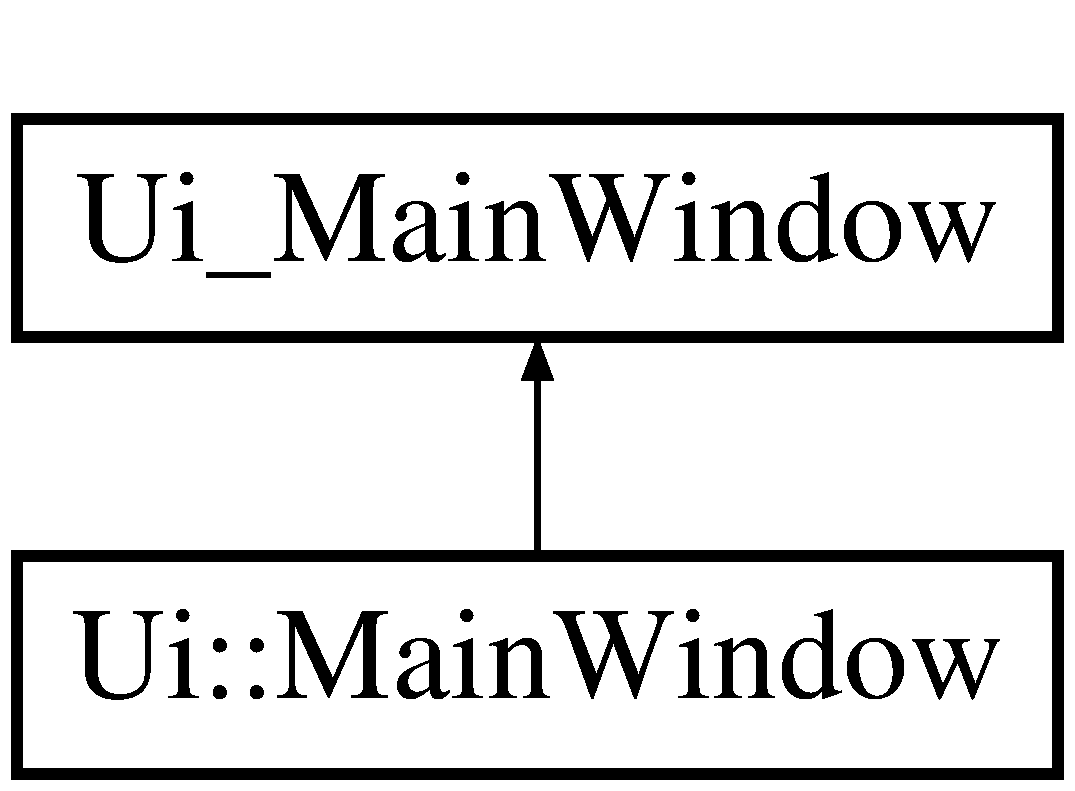
\includegraphics[height=2.000000cm]{class_ui_1_1_main_window}
\end{center}
\end{figure}
\subsection*{Additional Inherited Members}


The documentation for this class was generated from the following file\+:\begin{DoxyCompactItemize}
\item 
ui\+\_\+mainwindow.\+h\end{DoxyCompactItemize}

\hypertarget{class_main_window}{}\section{Main\+Window Class Reference}
\label{class_main_window}\index{Main\+Window@{Main\+Window}}
Inheritance diagram for Main\+Window\+:\begin{figure}[H]
\begin{center}
\leavevmode
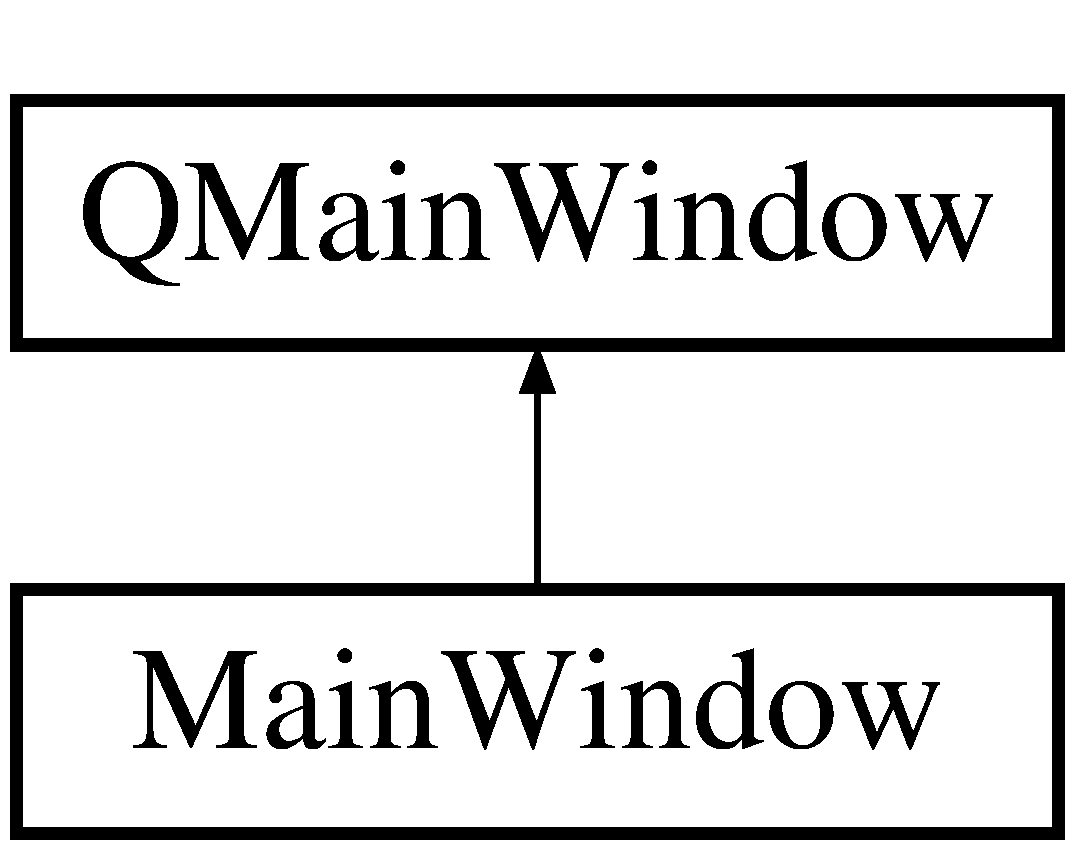
\includegraphics[height=2.000000cm]{class_main_window}
\end{center}
\end{figure}
\subsection*{Public Member Functions}
\begin{DoxyCompactItemize}
\item 
\mbox{\Hypertarget{class_main_window_a8b244be8b7b7db1b08de2a2acb9409db}\label{class_main_window_a8b244be8b7b7db1b08de2a2acb9409db}} 
{\bfseries Main\+Window} (Q\+Widget $\ast$parent=0)
\end{DoxyCompactItemize}


The documentation for this class was generated from the following files\+:\begin{DoxyCompactItemize}
\item 
mainwindow.\+h\item 
mainwindow.\+cpp\end{DoxyCompactItemize}

\hypertarget{class_ui___main_window}{}\section{Ui\+\_\+\+Main\+Window Class Reference}
\label{class_ui___main_window}\index{Ui\+\_\+\+Main\+Window@{Ui\+\_\+\+Main\+Window}}
Inheritance diagram for Ui\+\_\+\+Main\+Window\+:\begin{figure}[H]
\begin{center}
\leavevmode
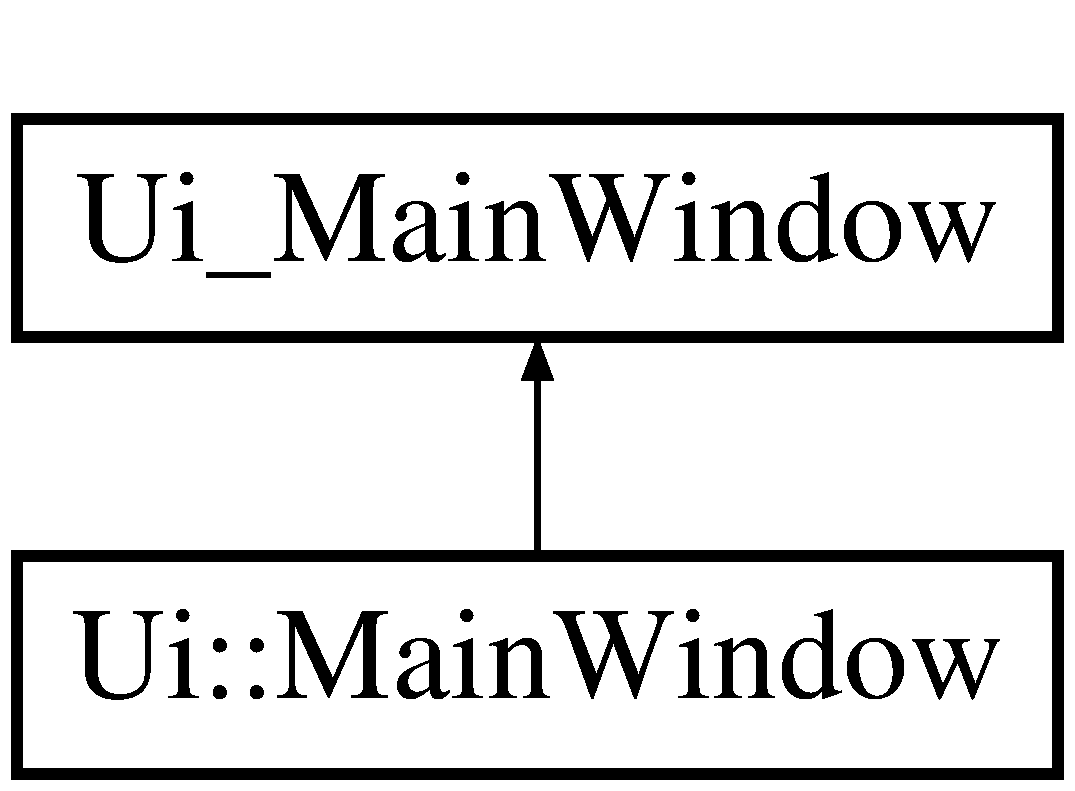
\includegraphics[height=2.000000cm]{class_ui___main_window}
\end{center}
\end{figure}
\subsection*{Public Member Functions}
\begin{DoxyCompactItemize}
\item 
\mbox{\Hypertarget{class_ui___main_window_acf4a0872c4c77d8f43a2ec66ed849b58}\label{class_ui___main_window_acf4a0872c4c77d8f43a2ec66ed849b58}} 
void {\bfseries setup\+Ui} (Q\+Main\+Window $\ast$\hyperlink{class_main_window}{Main\+Window})
\item 
\mbox{\Hypertarget{class_ui___main_window_a097dd160c3534a204904cb374412c618}\label{class_ui___main_window_a097dd160c3534a204904cb374412c618}} 
void {\bfseries retranslate\+Ui} (Q\+Main\+Window $\ast$\hyperlink{class_main_window}{Main\+Window})
\end{DoxyCompactItemize}
\subsection*{Public Attributes}
\begin{DoxyCompactItemize}
\item 
\mbox{\Hypertarget{class_ui___main_window_a30075506c2116c3ed4ff25e07ae75f81}\label{class_ui___main_window_a30075506c2116c3ed4ff25e07ae75f81}} 
Q\+Widget $\ast$ {\bfseries central\+Widget}
\item 
\mbox{\Hypertarget{class_ui___main_window_a525ed3c5fe0784ac502ee222fba4e205}\label{class_ui___main_window_a525ed3c5fe0784ac502ee222fba4e205}} 
Q\+Grid\+Layout $\ast$ {\bfseries grid\+Layout}
\item 
\mbox{\Hypertarget{class_ui___main_window_a2c789c07fa5fc1cee05aae8df52bb02d}\label{class_ui___main_window_a2c789c07fa5fc1cee05aae8df52bb02d}} 
Q\+Text\+Browser $\ast$ {\bfseries text\+Browser}
\item 
\mbox{\Hypertarget{class_ui___main_window_a2be1c24ec9adfca18e1dcc951931457f}\label{class_ui___main_window_a2be1c24ec9adfca18e1dcc951931457f}} 
Q\+Menu\+Bar $\ast$ {\bfseries menu\+Bar}
\item 
\mbox{\Hypertarget{class_ui___main_window_a5172877001c8c7b4e0f6de50421867d1}\label{class_ui___main_window_a5172877001c8c7b4e0f6de50421867d1}} 
Q\+Tool\+Bar $\ast$ {\bfseries main\+Tool\+Bar}
\item 
\mbox{\Hypertarget{class_ui___main_window_a50fa481337604bcc8bf68de18ab16ecd}\label{class_ui___main_window_a50fa481337604bcc8bf68de18ab16ecd}} 
Q\+Status\+Bar $\ast$ {\bfseries status\+Bar}
\end{DoxyCompactItemize}


The documentation for this class was generated from the following file\+:\begin{DoxyCompactItemize}
\item 
ui\+\_\+mainwindow.\+h\end{DoxyCompactItemize}

%--- End generated contents ---

% Index
\backmatter
\newpage
\phantomsection
\clearemptydoublepage
\addcontentsline{toc}{chapter}{Index}
\printindex

\end{document}
